\chapter{System Design}
When designing the system of the application the group had to adhere to the Ionic, and therefore Angular, way of design.

\section{Architechtural Model}
Angular JS uses an architecture model known as MVW (Model View Whatever). This is a term used mainly by Google when describing the Angular JS architecture.\cite{mvw} MVW is similar to MVC (Model View Controller) \cite{mvc} and MVVM (Model View ViewModel)  \cite{mvvm}but instead of having to use either a Controller or  a ViewModel one can use ``Whatever works for you".\\
\\
The system architecture the group chose to use was MVC (Model View Controller).
This is a fairly common architecture in mobile applications, as well as other platforms for software development where one wants to have changes in the view update the model and process them in the controller.
\\
\begin{figure}[h]
    \centering
    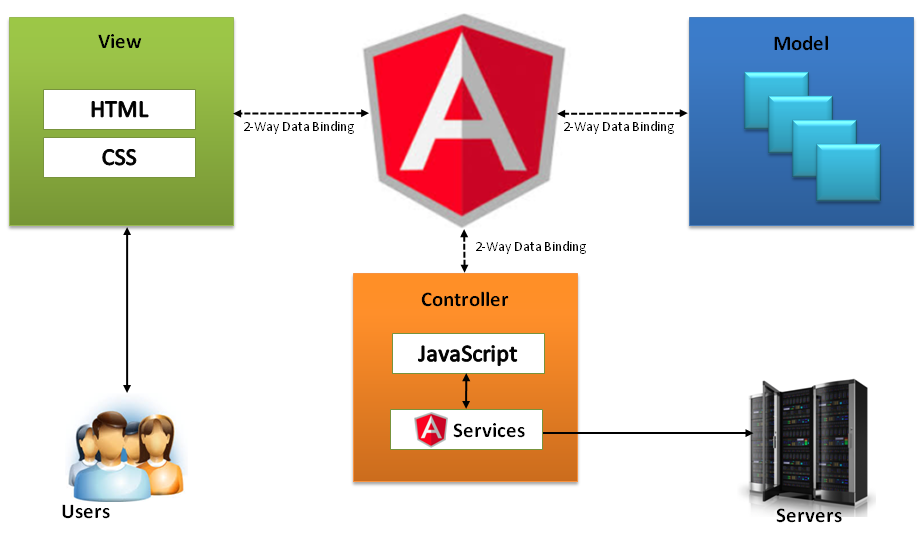
\includegraphics[scale=0.5]{images/MVC_angular.png}
    \caption{The AngularJS MVC architecture.}
    \label{fig:MVC}
\end{figure}
\\
As seen in figure \ref{fig:MVC}, The MVC architecture divides the system into three interconnected parts; Model, View and Controller.
The user interacts with the view (HTML) and changes the data (Model), calls the controller (interaction), Controller modifies the Model, interacts with Servers via services. AngularJS uses 2-way bindings to detect model changes and update the view. 
\\
\\
The view is what the user sees. It is the graphical interface that presents the data in the model. The view contains all buttons and other parts of the UI that creates interactivity. However, when this interactivity is activated the signal and information goes directly to the controller, which then decides what happens.
\\
\\
The controller is the part of the application that communicates with databases and transmits data between the modules of the application. It processes the data and sends it to the model, which updates the view with the given data. The controller can communicate directly with the view as well. This is usually done when no information is changed, for instance in the case of scrolling; all the information is already in the view, it is just not on the screen.
\\
\\
The model is responsible for editing and updating the information in the view. It receives data/information from the controller, stores it, and updates this in the part of the view where this is supposed to go.


\section{Implementation overview}
The system was implemented as a web-application running with some native functionality on either iOS or Android through the Cordova framework \cite{cordova2} which makes the web-application available offline as a normal application on smartphones. In addition to the normal web technology like HTML, CSS and JS the system used Angular JS, and Ionic Framework.

\subsection{Organization}
The project was organized first as a cordova application, with config files, plug-ins, and other application-building related files. The application's main project files are inside the ``www" folder. Common files are organized by file-type, and files for the different games inside its own folder called ``app".\\
\\
Each part of the game the group has made was separated into its own folder. Each part, referred to as an ``app" inside the game, has its own view and controller files. The view is a HTML template into which data is injected, parsed and read by the Angular controller.\\
\\
The application has a central module, ``routes.js", which decides which controller goes with which view, and in what structure they are. It is here that the inheritance is defined.\\\\
When ``compiled" our own JS files are concatenated into one big file, and the Ionic SCSS files compiled, which are then linked in \texttt{index.html}, which is the file first opened when starting the app.

\subsection{User interface}
The user interface views use inheritance to make reusable design possible. The design implementation uses tabs at the bottom or top of the screen, depending on the OS it runs in. Each of these tabs links to its own view which is displayed by default, from where one can explore the sub views if they exist. This can be seen in fig \ref{fig:tabs}.
\\
When going to sub-pages, your current ``position" is displayed at the top of the nav-bar, with a back button to take you back to the parent view.


\begin{figure}[!ht]
    \centering
    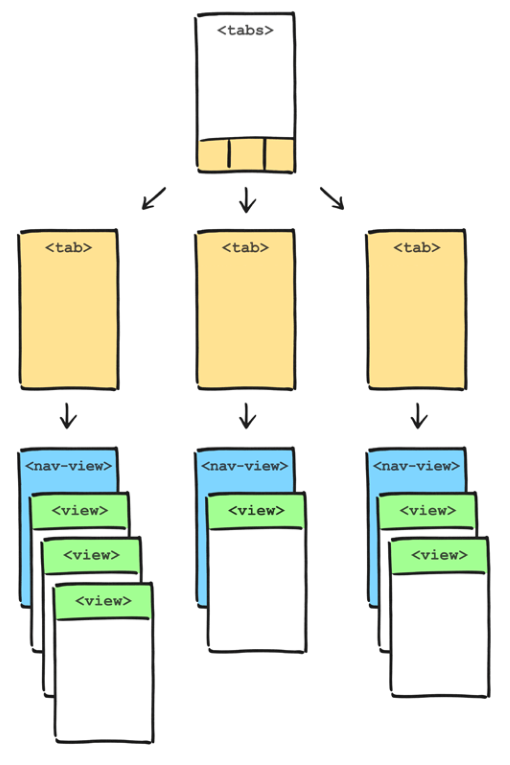
\includegraphics[scale=0.3]{images/tabviews.png}
    \caption{View structure in the Ionic tabs layout}
    \label{fig:tabs}
\end{figure}

\subsection{Frameworks}
Cordova is the fundamental part of the system, on top of which Ionic is implemented as a facilitator of structure and consistent design elements. Ionic uses Angular JS as a integral part of its workings \cite{ionic3} and can almost be said to be a angular project written as a plug-in for Cordova. When Ionic is run, Gulp compiles the SCSS code into normal CSS. The SCSS code gives us easy control over the overall look of the app, without having to change values throughout the groups entire style code.

\begin{figure}[h]
    \centering
    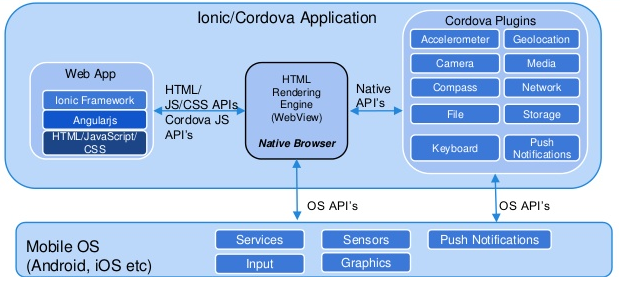
\includegraphics[scale=0.5]{images/mobile-app-architechure.png}
    \caption{Architecture of a normal Cordova application using Ionic}
    \label{fig:framework_architecture}
\end{figure}


\subsection{Controller}
Each sub-app of the application, either a minigame or another part of the game, has its own controller. The controller in Angular is a JS file with a unique controller name defined, which then is used in the view. The group used different function and variable scopes for different needs. Variables needed in the view are defined on the \$scope, while those which aren't are defined as normal ``var" variables. Variables which are used in other controllers are defined on \$rootScope.

\subsection{Model}
The group did not use a dedicated model in the traditional sense of the term, but uses globally defined variables with data such ass the game state and robot part configuration. These global variables are stored and synced to the device's LocalStorage store, where they will be stored even after the user closes the application. Any changes to these variables will immediately be stored in the LocalStorage to ensure that no data is lost. The implementation of this can be seen in ``www/js/app.js".\\\\
The application also uses a separate file for storing the translations of the different views, located in ``www/app/overview/translations.js". Due to the way Ionic concatenates files, the translations file had to be stored inside a sub-app's folder, not in a better suited location.

\subsection{View}
Each sub-app has its own view, a HTML document, which defines the structure and content which will be shown. Angular allowed the group to use dynamic elements in HTML, something which usually can't be done. Examples of this include using ``ng-repeat" which generates many similar elements from a scope variable, like when all the minigame buttons are generated from a minigame variable, and ``ng-class" which gave the group the possibility to automaticly change the style of elements based on the state of a game.\\\\
Translations are injected into the game by Angular by writing ``\{\{trans.TRANSLATION\_NAME\}\}", which meant that the group didn't have to handle the injection or changes of language themselves, since Angular changed all variables when the language was changed.

\subsection{Beacons}
In order to get beacons to work with the application, evothings-eddystone-plugin \cite{ibeacon_plugin} was used. It is a simple framework for reading beacon data. The functions used to read beacon data is found in  ``overviewCtrl.js" located in ``www/app/overview/OverviewCtrl.js". When the application starts, this file is initiated, and the application asks the user for permission to turn on Bluetooth. If permission is declined, and bluetooth can not be used, an error is thrown. This is handled by setting a boolean value ``beaconsActive" to false, and makes the application use the backup solution. With beaconsActive set to false, the application goes into the backup solution, which means the user can play all the minigames without them being unlocked by a beacon on a specific location.

\section{Backend}
The backend of the project is necessary to keep submitted robots in a central place. This was solved by having a simple script on Vitensenteret's servers, which take submitted robots, store them, and display them.

\subsection{Functionality}
When a player has collected all robot parts, he has the possibility of naming and uploading the robot to Vitensenteret's servers, where it will be shown alongside other people's robots, like a ``hall of fame". See \ref{fig:robots_backend}.

\begin{figure}[H]
    \centering
    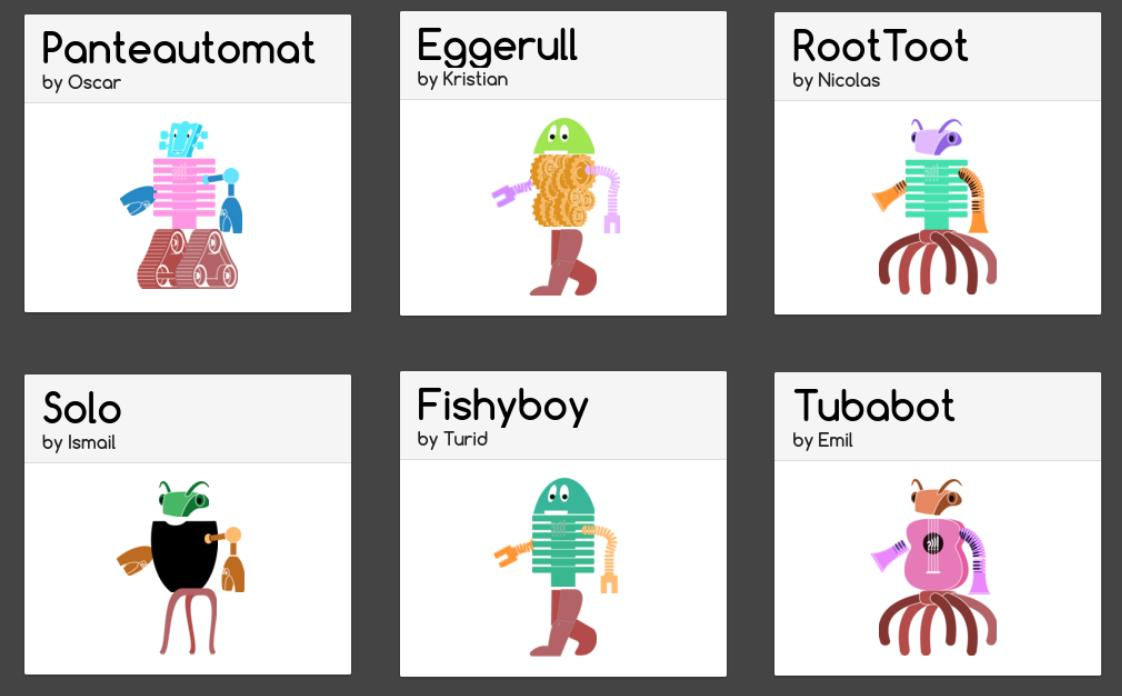
\includegraphics[width=0.5\textwidth]{images/app/robots_backend.jpg}
    \caption{Screenshot of the Robot Hall of Fame}
    \label{fig:robots_backend}
\end{figure}


\subsection{Storage and Models}
The robot model consists of the robot's name, given by a player, the player's name and the robot parts selected and customized by a player.r. 
As the robot part data is taken directly from the mobile app it contains some non-relevant data, for example if the part has been collected or not. 
This does not occupy much space and simplifies the job of sending the data to the server. The parts object contains 5 dictionaries, one for each body part, each of which contains the part's name, which variation on that part has been chosen and the hue and lightness of the part.
\\
\\
The data is stored in a JSON format and file by the PHP script running on the server. This storage method was chosen because the group had no guarantees of what the server environment would look like, or if the group had access to MYSQL or anything else. The format is sufficient for our very simple use, and can be easily replaced with MySQL in the future if there ever arises a need to supervise and manage the data.

\subsection{Implementation}
The backend is a simple stand-alone Angular and PHP site, which can either recieve a new robot request from the mobile app, or display all existing robots.
\\
\\
When the app recieves a robot it gets the robot's name, creator's  name and robot parts from the POST request the mobile app made. The robot parts are JSON encoded dictionaries or objects, which the PHP script checks and stores.
\\
\\
When the server is going to show all robots, PHP is not used at all. The Angular app retrieves a JSON file with all the robots stored in it, imports it, and shows each robot using the exact same code (CSS, HTML and JS) that the mobile app uses, so that the robot is displayed consistently across different platforms. This also means that updates to the robot displaying code or design can be integrated into the backend quickly without having to adapt the code.


